\documentclass{suturo}
\usepackage[utf8]{inputenc}
\usepackage{listings}



\begin{document}
    \maketitle{Suturo}{02.01.2017}{}{1}{}{}{}{}

\makeatletter
\newcommand{\chapterauthor}[1]{%
  {\parindent0pt\vspace*{-27pt}%
  \linespread{0}\small\begin{flushright}von: #1\end{flushright}%
  \par\nobreak\vspace*{0pt}}
  \@afterheading%
}
\makeatother


\section{Einleitung}
\subsection{Vorwort}
\chapterauthor{Kevin Störmer}
Im Rahmen unserer Bachelorprojektarbeit 'Suturo', haben wir die Chance ein intelligentes Robotersystem, am Roboter 'Pr2' von Willow Garage zu entwickeln. \\
Dabei wurde in Absprache mit unseren Tutoren, eine Zielsetzung entwickelt, die wir im Rahmen des letzten Meilensteines verfolgt haben, aufbauend auf unseren Erfolgen des vorherigen Meilensteines. \\
In den Folgenden Abschnitten wollen wir allem vorran einleitend auf planende Aspekte, sowie unsere Vorgehensweisen und Zielsetzungen eingehen. Daraufhin soll im Abschnitt zu unserer Schnittstellendokumentation, auf konkrete Lösungen der Projektgruppen eingegangen werden.\\ ~ \\
Abschliessend wollen wir einen Ausblick auf kommende Meilensteine, insbesondere im Hinblick auf die im April folgende Projektpräsentation, formulieren.\\
Eine Installationsanleitung finden sie im letzten Abschnitt unserer Dokumentation.

\newpage

\subsection{Zielsetzung}
\chapterauthor{Kevin Störmer}
\subsubsection{Prämisse}
\begin{itemize}
\item Der Pr2 befindet sich beliebig im Raum zwischen Küche und Küchenzeile.
\item Auf der Küchenzeile befindet sich eine beliebige Anzahl Gegenstände aus einer festgelegten Menge. (Tomatensoße, Ja-Milch, Pringles-Salt, Pringles-Paprika, Edeka-Schüssel, Hella Curryketchup, Müsli usw)
\item Es befinden sich keine Fremdkörper auf dem Boden der Küche, oder im Arbeitsbereich des Pr2.
\end{itemize}

\subsubsection{Ablauf}
\begin{itemize}
\item Der Pr2 fährt in Home-Position, dh. die Arme des Pr2 werden über den Kopf gefahren, und der Pr2 bewegt seine Basis in eine feste Position vor der Küchenzeile.
\item Der Roboter fährt mit deinem Kopf eine Reihe festgelegter Punkte, anhand der Küchenzeile entlang.
\item Nach jedem mit dem Kopf gefahrenen Schritt, versucht der Pr2 Objekte zu entdecken. 
\item Entdeckte Objekte werden an die Wissenzentrale des Pr2 weitergeleitet und anhand eines Classifiers identifiziert.
\item Die Wissenzentrale entscheidet, welche der gesehenen Objekt gegriffen werden sollen.
\item Der Pr2 greift mit dem am besten geeigneten Gripper das gesuchte Objekt. 
\item Befindet sich kein weiteres Objekt im Sichtfeld, bewegt der Pr2 seinen Kopf weiter. 
\item Entdeckt der Pr2 nun ein weiteres Objekt, wird es mit dem freien Gripper gegriffen.
\item Ist ein Objekt für den Pr2 nicht greifbar, versucht der Roboter durch geschicktes Umpositionieren der Basis das Objekt zu greifen.
\item Sind beide Gripper des Pr2s gefüllt, wird in der Wissensbasis erfragt, an welchen Platz diese Objekt positioniert werden sollen.
\item Der Roboter bewegt seine Basis so nah an die Ablegeposition eines der Objekte, wie möglich.
\item Der Roboter bewegt seinen Gripper so, dass das Objekt an der vorgesehenen Stelle abgelegt wird.
\item Ist ein Platz bereits belegt, wird das Objekt an eine freie Stelle innerhalb der Zone abgelegt.
\item Nun wird das Objekt im anderen Gripper an seine vorgesehene Position gebracht
\item Dies wird solang wiederholt bis die Küchenzeile leer ist.
\item Sollte im laufe der Fahrt ein Gegenstand aus dem Gripper des Pr2 fallen, oder sollte der Pr2 fälschlicherweise glauben beide seiner Gripper seien gefüllt , unterbricht der Pr2 seine Arbeit.
\item Der Pr2 nimmt, nach Freigabe eines Menschen, seine Aufgabe wieder auf. Beginnt also damit, seine leeren Gripper zu füllen.
\end{itemize}


\subsubsection{Abschluss}
\begin{itemize}
\item Die Küchenzeile ist leer.
\item Alle Objekte, welche ehemalig auf der Küchenzeile standen, befinden sich in den vorgesehenen Bereichen.
\item Der Pr2 befindet sich in Home-Position
\end{itemize}
\subsection{Aufgabenverteilung}
\chapterauthor{Kevin Störmer}
\subsection{Probleme}
\chapterauthor{Kevin Störmer}



%drinlassen?
\newpage
    \maketitle{Planning}{03.03.2018}{}{1}{}{}{}{}



\section*{Zielsetzung}
Das Ziel von Gruppe Planning im zweiten Meilenstein ist zu einem die Kommunikationsschnittelle zwischen den anderen Gruppen zu sein, aber auch eigene wichtige Funktionalitäten hinzuzufügen. Planning selber ist für das Fahren zwischen den Tischen, das Errorhandling wenn ein Objekt nicht gegriffen werden kann oder runterfällt, sowie das Entscheiden wo ein Objekt genau hingestellt werden soll zuständig.
 

\section*{Probleme}
\subsection*{Routen können nicht richtig geplant werden}
\chapterauthor{Vanessa Hassouna}
Beim fahren fährt der Roboter schnell mit seinen Armen gegen Küchenobjekte und dreht sich in einem Winkel der problematisch mit seinem verletzbaren Rücken ist.\\


\textbf{Lösung}: Bevor er zu dem gegeben Punkt fährt, fährt er in eine von uns ausgewählte sichere Position. Bis dahin sollte er sich um 90 Grad gedreht haben.

\subsection*{Extrahieren von wichtigen Information}
\chapterauthor{Vanessa Hassouna}
Bei dem Erhalt von Vision über die Informationen der gesehenen Objekte kommt eine sehr unübersichtliche \textbf{msg} die zerlegt werden muss. Hier kann es schnell zu Fehlern kommen, wenn man die Information als globale Variablen speichert. \\

\textbf{Lösung}: Alle erhaltenen Informationen werden zwischengespeichert auf dem Param-Server, danach werden dieses erst miteinander konkateniert.

\subsection*{Logik der Main wird zu groß und unübersichtlich}
\chapterauthor{Vanessa Hassouna}
Für eine sinnvolle Logik der Main ist eine gute Übersicht zu schaffen. Da die Logik der Main jedoch immer fulminanter wird passieren hier schnell Fehler.\\

\textbf{Lösung}: Die Logik der Main wurde in mehrere Teilabschnitte getrennt und in neue Funktionen geschachtelt. Eine weitere Schnittstelle \textbf{planning\_logic} dient zur Extraktion von logischen Zwischenabschnitten.


\section{Die Quellcode-Datei: main.lisp (planning\_main\_programm)}
\subsection{Architekturbild}
\chapterauthor{Kevin Störmer}


\begin{figure}[!htb]
        \center{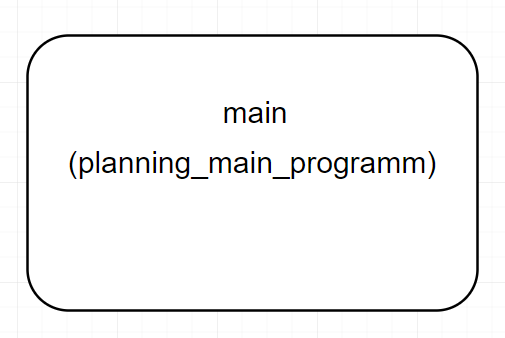
\includegraphics[width=0.4\textwidth]
        {img/diag_planning_main_programm.png}
        \caption{} Architektur der Quellcode-Datei main.lisp}
\end{figure}
      


\subsection{Beschreibung des Teilsystems}
\subsubsection{\"Ubersicht}
\chapterauthor{Kevin Störmer}
Die Die Quellcode-Datei 'main' im Paket 'planning\_main\_programm' soll ausschliesslich auf höchster Ebene den internen Ablauf des PR2 modellieren. 

Alle dafür notwendigen Logiken, die auf Basis externer Daten entschieden werden, wurden dabei basierend auf der Quelle der Daten in andere Die Quellcode-Dateien ausgelagert. Dabei wurde z.b der Vergleich zweier Punkte aus Vision in die Die Quellcode-Datei 'points' (Paket: planning\_vision) ausgelagert.


\subsubsection{main()}
\chapterauthor{Vanessa Hassouna}


\noindent
\begin{minipage}{\linewidth}
\begin{lstlisting}
(defun main ()
  "Main function - Executing and planning robot behaviour on the top level"
  (roslisp:with-ros-node ("planning_main")
(roslisp::ros-info "Main" "Robotlife seems hard, but lets do this")
[...]
\end{lstlisting}
\end{minipage}

Die Main startet eine 'ros-nod' mit dem Namen \textit{planning\_main}. Diese node läuft solange, komplette Main einmalig durchlaufen wurde.

\section*{Programmablauf}
\chapterauthor{Vanessa Hassouna}
\subsection*{Schritt 1: Vorbereiten des Roboters}
Der Pr2 begibt sich in die Homeposition von der aus er Objekte sehen soll. 

\subsection*{Schritt 2: Suche nach Objekten}
Jedes mal, wenn der Kopf in einer Position ist wird der Service \textit{/vision\_suturo/objects\_information} aufgerufen. Die gegeben Information werden wie folgt bearbeitet:

\begin{itemize} 
\item Die Informationen werden extrahiert.
\item Die beiden Arrays normal\_features und color\_features werden auseinander genommen und mithilfe von object\_amount auf dem Param-Server gespeichert mit der Nummer des Objektes zu der Identifikation.
\item Die normal\_features und color\_features werden konkateniert auf dem Param-Server gespeichert als "featuresX", wobei X hier die Nummer des Objektes darstellt.
\item Die Posen werden als Array global gespeichert.
\end{itemize}


\subsection*{Schritt 3: Weitergabe} 

\begin{itemize} 
\item Jetzt werden die gesehenen Objekte weitergeben an Knowledge, hier bekommen wir für jedes gegebene Objekt ein Label als String zurück.
\item Mit hilfe des erhaltenen Labels rufen wir einen anderen Service von Vision auf der Anhand von Objekt-Nummer und Label uns eine Pose zurück gibt.  
\item Wenn die Pose bei uns angekommen ist publishen wir auf ein Topic von Knowledge damit das gesehene Objekt in der Wissensbasis gespeichert wird.
\end{itemize}



\subsection*{Schritt 4: Welches Objekt soll ich greifen und wo soll es hin}
Wir erfragen bei Knowledge welche Objekte wir greifen sollen.
Mit der Funktion X kriegen wir dann einen Standpunkt raus wo das Objekt hin soll. %X=Haukesfunktion Name muss hier noch ergäntzt werden
Des weiteren wird noch abgefragt wie das Objekt gegriffen werden, soll. Die Information wird dann weiter an Motion gegeben.

\subsection*{Schritt 5: Hinfahren zum gegebenen Ort}
Mit Hilfe des Punktes wird berechnet wo der Roboter hinfahren muss. 
 
\subsection*{Schritt 6: Abstellen und weiter}
Das Objekt wird abgestellt.
Danach fährt der Pr2 wieder zu seiner Homeposition und sucht die nächsten Objekte.






%
%
%\subsubsection{find-Object (x z)}
%\chapterauthor{Vanessa Hassouna}
%Die Funktion find-Object im Paket 'planning\_move' lässt den Pr2 genau \textbf{8} verschiedene Zustände durchlaufen. Dieses Vorgehen endet entweder wenn ein Objekt gefunden wurde, oder gegebenenfalls alle 8 Zustände erfolglos durchlaufen wurden.
%
%\noindent
%\begin{minipage}{\linewidth}
%\begin{lstlisting}
%(defun find-Object (x z)
% "Looking around from 2 to -2 to find an object"
%(let ((positions (make-array '(8) 
%   :initial-contents '(0.0 0.5 1 1.5 2.0 -0.5 -1.5 -2.0))))
%  (loop for i across positions do
%    (progn
%      (let ((y i))
%        (move-Head x y z))
%      (if (planning-move::ask-For)
%          (progn
%            (roslisp::ros-info "find-Object" "I found an object, lets move on ")
%            (return-from find-Object T))
%          (roslisp::ros-info "find-Object" "I can't find any object, let me try it again")))))
%(return-from find-Object nil))
%\end{lstlisting}
%\end{minipage}
%
% Die als Parameter übergebenen \textbf{X-} und \textbf{Z-Werte} sind festgelegt und ändern sich nicht mehr in der Funktion. Der Kopf wird hier mit der oberen Funktion move-Head bewegt. Der einzige Wert der also verändert wird ist der \textbf{Y-Wert}.\\
%
% Dieser führt dazu, dass der Punkt sich im Koordinatensystem (ausgehend von dem \textit{base\_link} 'frame') so verändert, dass der Pr2 nach links und rechts guckt. Die Zustände werden hier in einem Array gespeichert. Dieses Array wird durchlaufen und der jeweilige gespeicherte Wert in einer Zelle wird der Funktion move-Head (planning\_move) als \textbf{Y-Wert} übergeben (mit den Parametern die find-Object selber übermittelt bekommt).Dann wird die Funktion askFor aus dem Paket 'planning\_move' aufgerufen, jene liefert true oder false zurück wie oben beschrieben.\\
% 
% Wenn also ein Objekt gefunden wurde wird eine positive Nachricht ausgegeben und ebenso eine negative für den gegenteiligen Fall.
%  Wurden alle Zustände erfolglos angenommen liefert die Methode ein \textbf{false} zurück.
  



\newpage
\section{Die Quellcode-Datei: vision\_communicate.lisp (planning\_vision)}

\subsection{Architekturbild}

\chapterauthor{Vanessa Hassouna}



\begin{figure}[!htb]
        \center{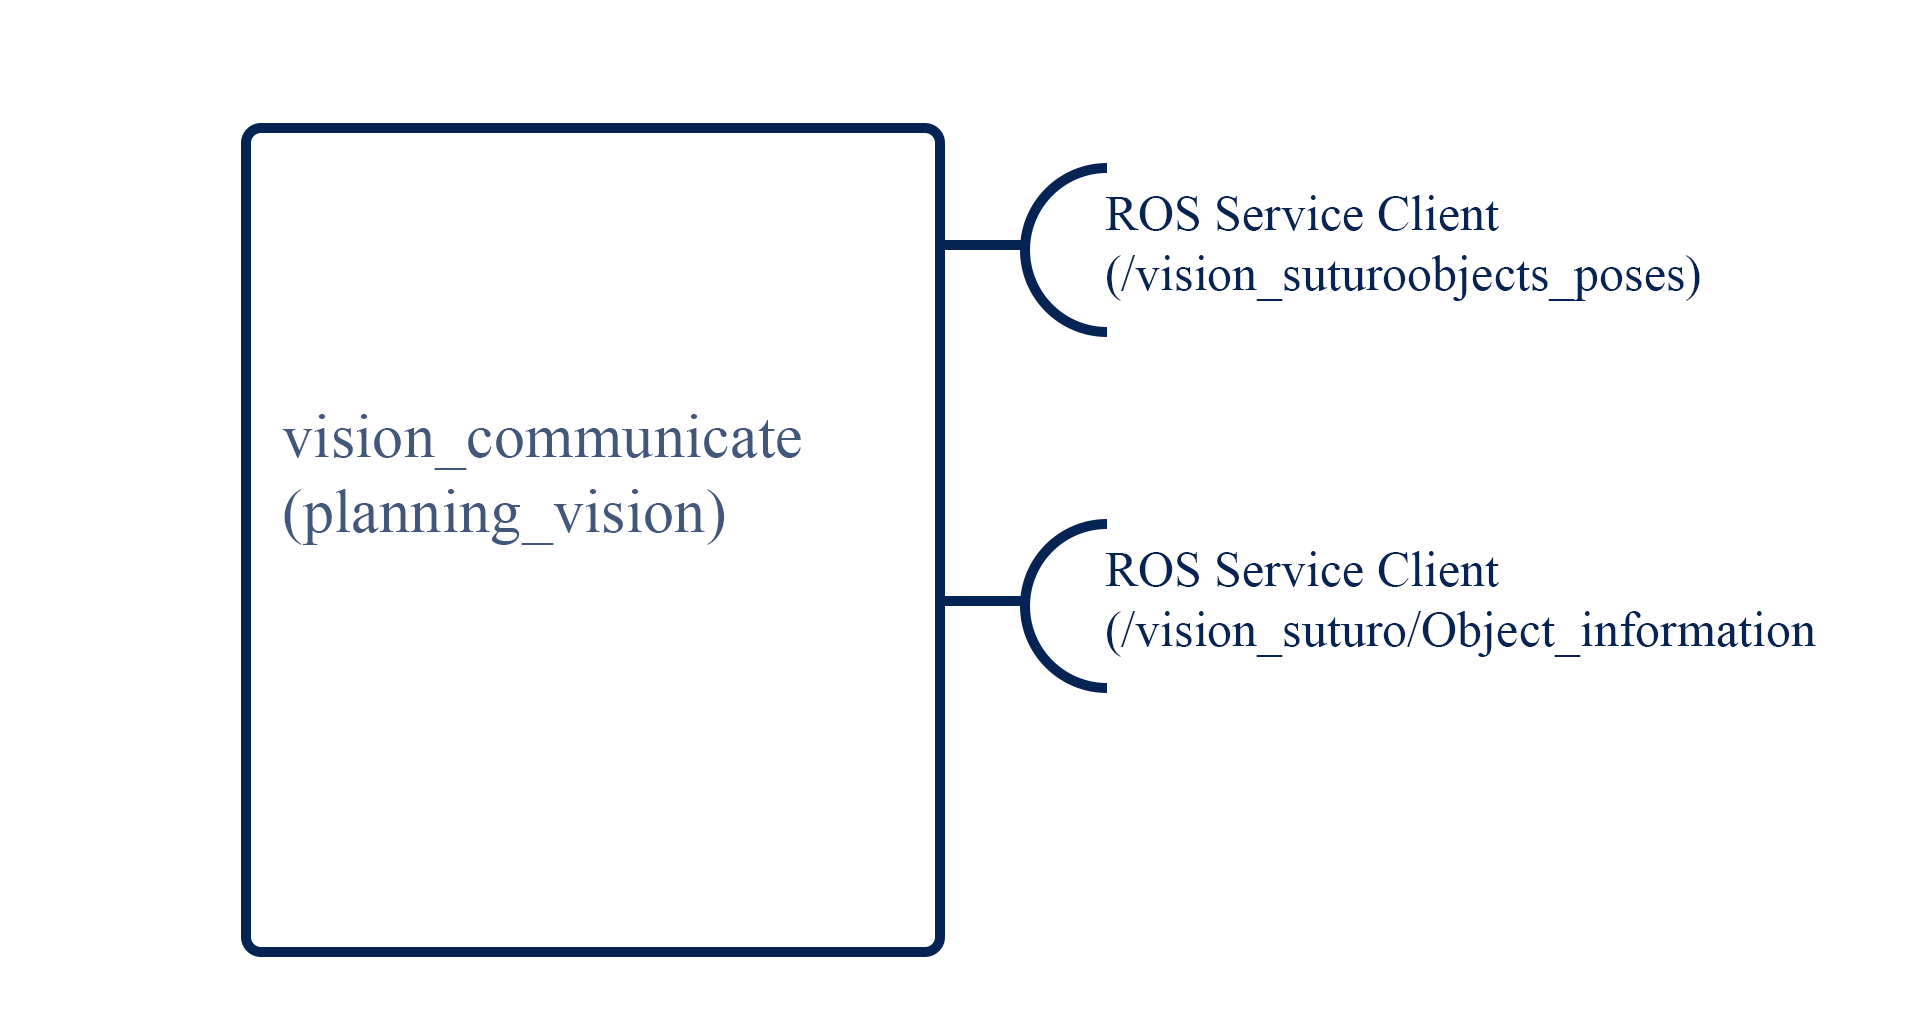
\includegraphics[width=0.6\textwidth]
        {img/vision.png}
        \caption{} Architektur der Quellcode-Datei vision\_communicate.lisp}
\end{figure}


\subsection{API}
\chapterauthor{Vanessa Hassouna}
\subsubsection{Serviceclients}
1. '/vision\_suturo/Object\_information' \\
Nimmt Objekt über Kinect wahr, und gibt eine "msg" zurück die Colorfeatures, Normalfeatures, Objectamount und Pose beinhaltet.\\ \\
2. '/vision\_suturo/objects\_pose' \\
Gibt zu einem Objekt (übergeben als Nummer) und einem Label (übergeben als String) die Pose mit Rotation zurück.

\subsection{Beschreibung des Teilsystems}


%willst du die noch einmal überarbeiten?
%In der aktuellen Version funktoniert sie nicht.
\subsubsection{check-points-is-equal (msg-one msg-two delta)}
\chapterauthor{Kevin Störmer}

\noindent
\begin{minipage}{\linewidth}
\begin{lstlisting}
(defun check-points-is-equal (msg-one msg-two delta)
  "Compares two points with delta."
  (roslisp::ros-info "check-points-is-equal" "Starting to check if point of object is still valid")
  (roslisp:with-fields ((x1 (geometry_msgs-msg:x geometry_msgs-msg:point)) 
                        (y1 (geometry_msgs-msg:y geometry_msgs-msg:point))
                        (z1 (geometry_msgs-msg:z geometry_msgs-msg:point)))
     (object_detection-msg:position (object_detection-srv:object msg-one))
     (roslisp:with-fields ((x2 (geometry_msgs-msg:x geometry_msgs-msg:point)) 
                           (y2 (geometry_msgs-msg:y geometry_msgs-msg:point))
                           (z2 (geometry_msgs-msg:z geometry_msgs-msg:point)))
                        (object_detection-msg:position (object_detection-srv:object msg-two))
       (let (
             (dx (abs (- x1 x2)))
             (dy (abs (- y1 y2)))
             (dz (abs (- z1 z2)))
             )
         (if (and
              (<= dx delta)
              (<= dy delta)
              (<= dz delta)
              )
             (print t)
             (print nil)
             )
         )
       )
    )
  )
\end{lstlisting}
\end{minipage}

Die Funktion 'check-points-is-equal' bekommt die Parameter 'msg-one' und 'msg-two' \"ubergeben. Dabei handelt es sich um Messages vom Typ 'object\_detection-msg'. Diese enthalten Punke (x, y, z) die zu verschiedenen Zeiten von Vision über die Kinect wahrgenommen wurden. Sie stellen den Mittelpunkt des umzustossenden Objektes dar. Beim \"Ubergabeparameter delta, handelt es sich um die maximale erlaubte Tolleranz mit der die beiden Punkte von einander abweichen dürfen. \\
Anf\"anglich werden die Koordinaten der beiden Messages aus den Wrappern extrahiert und in Variablen fortan verf\"ugbar gemacht. Danach werden die Koordinaten paarweise voneinander subtrahiert um die Differenz beider als vorzeichenlose Zahl zu errechnen. Diese Differenz wird dann mit dem vorgegebenen Delta verglichen. Wenn sich alle Differenzen innerhalb des Deltas befinden, wird 'true' zurückgegeben, sonst 'nil'. 

\noindent
\begin{minipage}{\linewidth}

%Rausschmeisen? In der aktuellen Version wird diese Methode nicht verwendet und funktoniert auch nicht mehr.
\subsubsection{call-vision-point ()}
\chapterauthor{Hauke Tietjen}
\begin{lstlisting}
(defvar not-a-number)

(defun call-vision-point ()
  "Call vision service, to look for point. Returns ObjectDetection object"
  (cpl:with-retry-counters ((retry-counter 10))
    (cpl:with-failure-handling
        ((cpl:simple-plan-failure (error-object)
           (format t "An error happened: ~a~%" error-object)
           (cpl:do-retry retry-counter
             (format t "Now retrying~%")
             (cpl:retry))
           (format t "Reached maximum amount of retries. Now propagating the failure up.~%")))
      (let ((response
              (roslisp:call-service
               "/vision_main/objectPoint"
               'object_detection-srv:visobjectinfo)))
        ;;Debug to find NaN message from vision
        (setf not-a-number response)
        (print not-a-number)
        (roslisp:with-fields ((x (geometry_msgs-msg:x geometry_msgs-msg:point)) 
                              (y (geometry_msgs-msg:y geometry_msgs-msg:point))
                              (z (geometry_msgs-msg:z geometry_msgs-msg:point)))
            (object_detection-msg:position (object_detection-srv:object response))
          ;;If Vision returns a NaN and it is of type String this will recover from the error
          (if (or (stringp x)
                  (stringp y)
                  (stringp z))
              (cpl:fail "One or more of the coordinates returned by the service /vision_main/objectPoint is of type String
                        which is likely the not a number error")
              (if (or (sb-ext:float-nan-p x)
                      (sb-ext:float-nan-p y)
                      (sb-ext:float-nan-p z))
                  (cpl:fail "One or more of the coordinates returned by the service /vision_main/objectPoint is  not a number")
                  (roslisp:with-fields (object_detection-msg:error) (object_detection-srv:object response)
                    (if (or (string= "Cloud empty. " object_detection-msg:error)
                            (string= "Cloud was empty after filtering. " object_detection-msg:error)
                            (string= "No plane found. " object_detection-msg:error)
                            (string= "Final extracted cluster was empty. " object_detection-msg:error))
                        (cpl:fail (concatenate 'string "Service call failed: " object_detection-msg:error))
                        (progn
                          (format t "Service call successful.")
                          (return-from call-vision-point
                            (roslisp:call-service "/vision_main/objectPoint" 'object_detection-srv:VisObjectInfo))))))))))))
\end{lstlisting}
\end{minipage}

Die Funktion 'call-vision-point' ruft den Service '/vision\_main/objectPoint' von Vision auf. Dieser Service gibt den Mittelpunkt des gesehenen Objekts zurück welcher dann nach einer Fehlerüberpüfung als 'object\_detection-msg' zurückgegeben wird. 

In Gazebo gibt dieser Service manchmal ein 'not a number' zurück, daher wird der Rückgabewert daraufhin überprüft. Es ist noch nicht klar ob 'NaN' als String oder float übergeben wird, daher wird beides überprüft. Zu 'sb-ext:float-nan-p' muss man sagen das es überprüft ob die nachfolgende Variable ein 'NaN' enthält und falls ja 't' zurückgibt, weil dazu keine Dokumentation auffindbar ist. Dann werden noch die bereitgestellten Fehlermeldungen von Vision abgefragt, z.B. ob überhaupt ein Objekt gesehen wurde. Falls mindestens eine dieser Abfragen zutrifft wird der Service-Call und die Fehlerüberprüfung neu gestartet. Dadurch kann die Funktion bis zu zehn mal neu gestartet werden bis sie endgültig aufgibt. Hier könnte in Zukunft eine Funktion auf höherem Level anknüpfen und den Kopf oder den ganzen Roboter bewegen um das Objekt doch noch zu erkennen.


\subsubsection{call-Vision-Object-Clouds ()}
\chapterauthor{Vanessa Hassouna}
\begin{verbatim}
call-Vision-Object-Clouds ()

Beschreibung: Der Service von Vision  "/vision\_suturo/objects\_information" wird
aufgerufen.

@return: Succesfull oder Aborted
\end{verbatim}






%%%%%%%%%%%%%%%%%%%%%%%%%%%%%%%%%%%%%%%%%%%%%%%%%%%%%%%%%%%%%%%%%%


\section{Die Quellcode-Datei: knowledge-communicate.lisp\\
 (planning\_knowledge)}
\subsection{Architekturbild}
\chapterauthor{Vanessa Hassouna}

\begin{figure}[!htb]
        \center{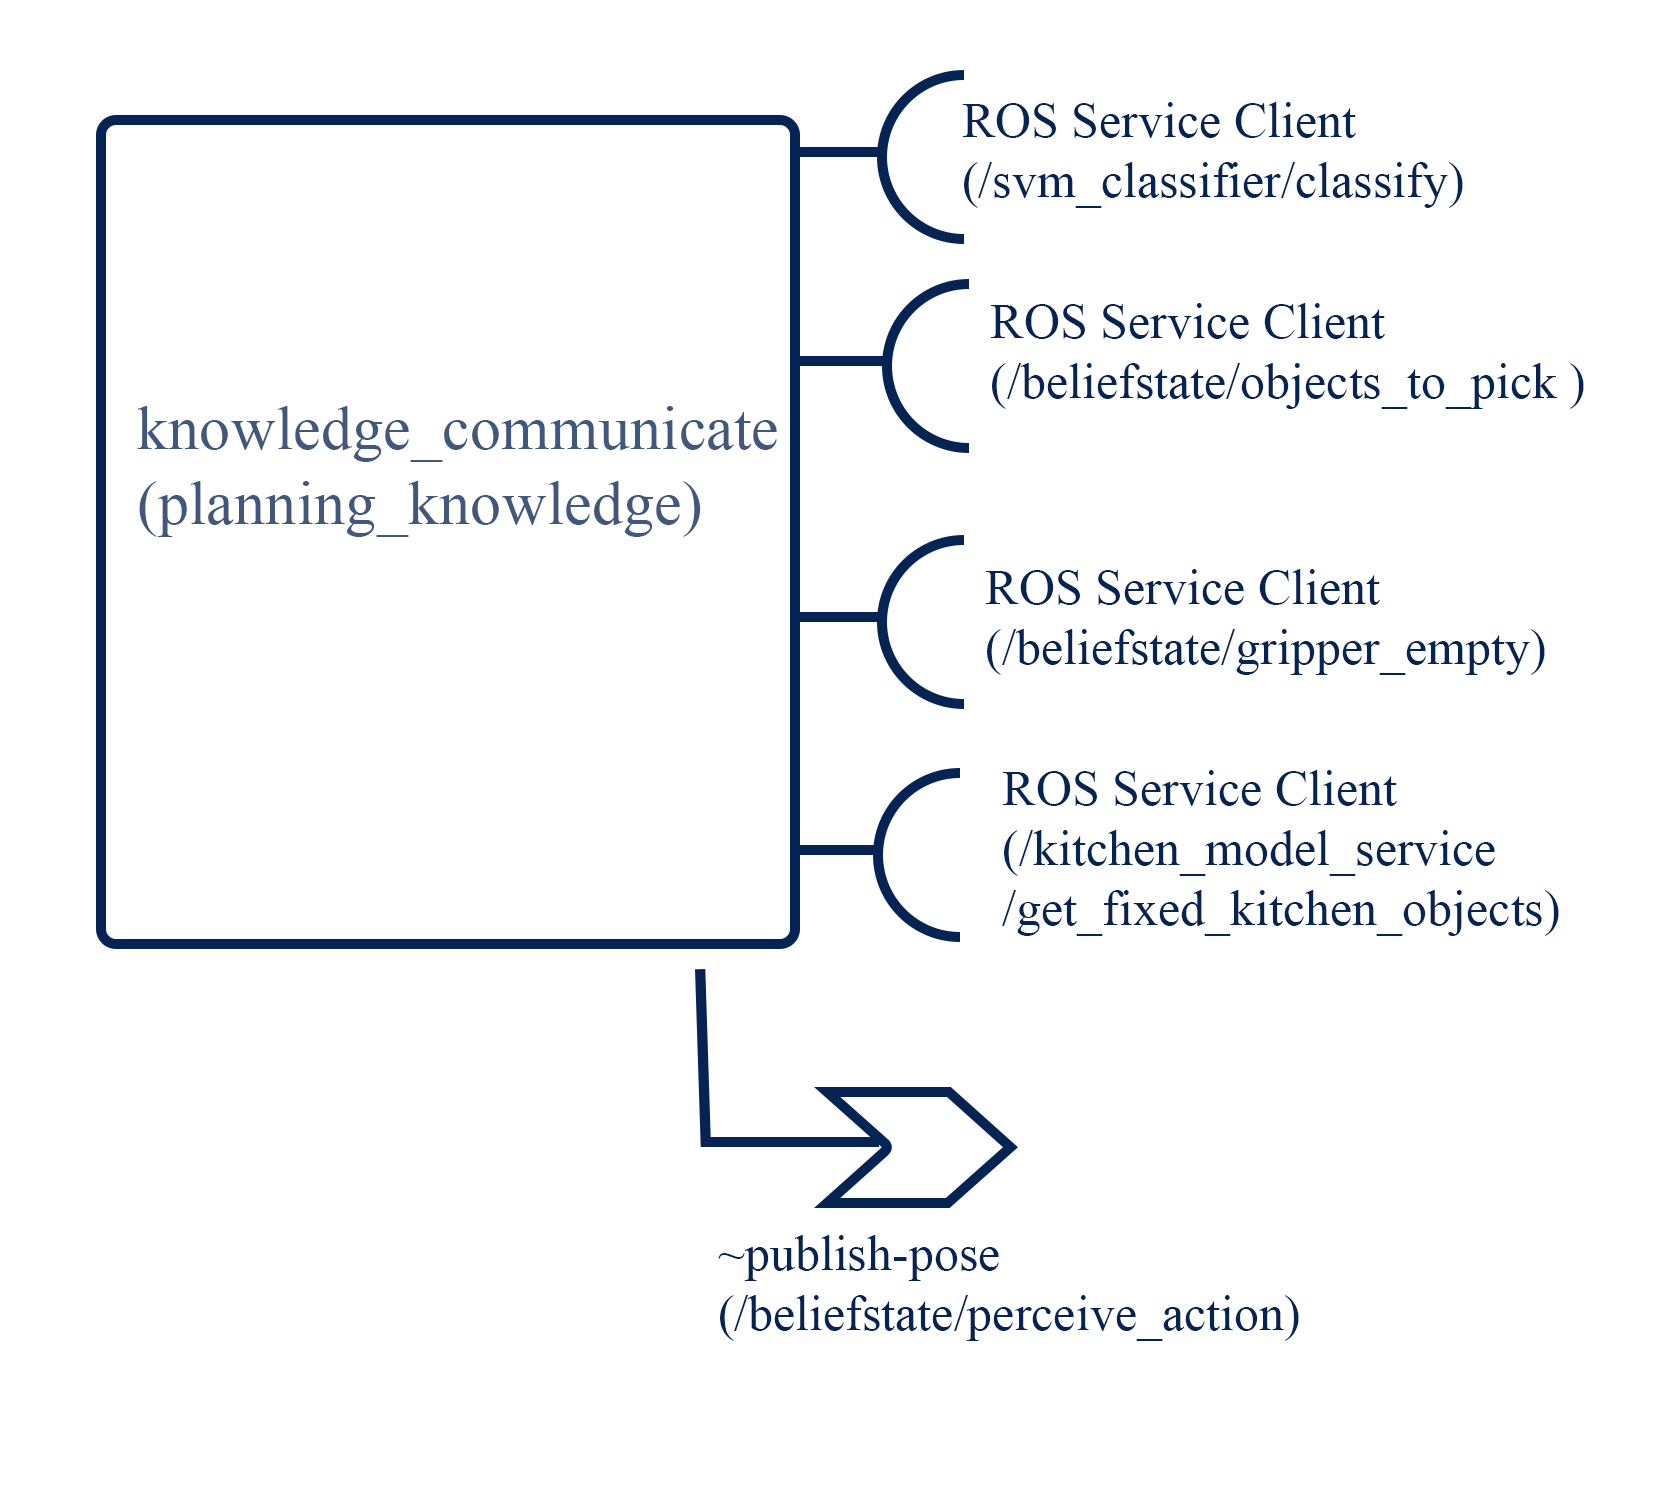
\includegraphics[width=0.6\textwidth]
        {img/knowledge.png}
        \caption{} Architektur der Quellcode-Datei knowledge-communicate.lisp}
\end{figure}

\subsection{API}
\chapterauthor{Vanessa Hassouna}
\subsubsection{Serviceclients}
1. 'svm\_classifier/classify' \\
Gibt uns ein Label als String für ein Objekt zurück.\\

2. 'beliefstate/objects\_to\_pick'\\
Gibt uns eine 0-2 Strings zurück, welche Objekte gegriffen werden sollen.\\

3. 'beliefstate/gripper\_empty'\\
Wir können erfragen welcher Gripper frei ist.\\

4. 'kitchen\_mode\_service/get\_fixed\_kitchen\_objects'\\

\subsubsection{Topics}
1. 'beliefstate/perceive\_action'\\
Wenn ein Objekt wahrgenommen wurde, geben wir die Information weiter.


\subsection{Beschreibung des Teilsystems}
\subsubsection{\"Ubersicht}
\chapterauthor{Kevin Störmer}
Die Die Quellcode-Datei 'knowledge-communicate' im Paket 'planning\_knowledge' ist ausschliesslich für die Kommunikation mit Gruppe Knowledge zust\"andig.

%%%%%%%%%%%%%%%%%%%%%%%%%%%%%%%%%%%%%%%%%%%%%%%%%%%%%%%%%%%%%%%%%%%%%%%%%%%%%%

\section{Die Quellcode-Datei: motion-actions.lisp (planning\_motion)}
\subsection{Architekturbild}
\chapterauthor{Vanessa Hassouna}


\begin{figure}[!htb]
        \center{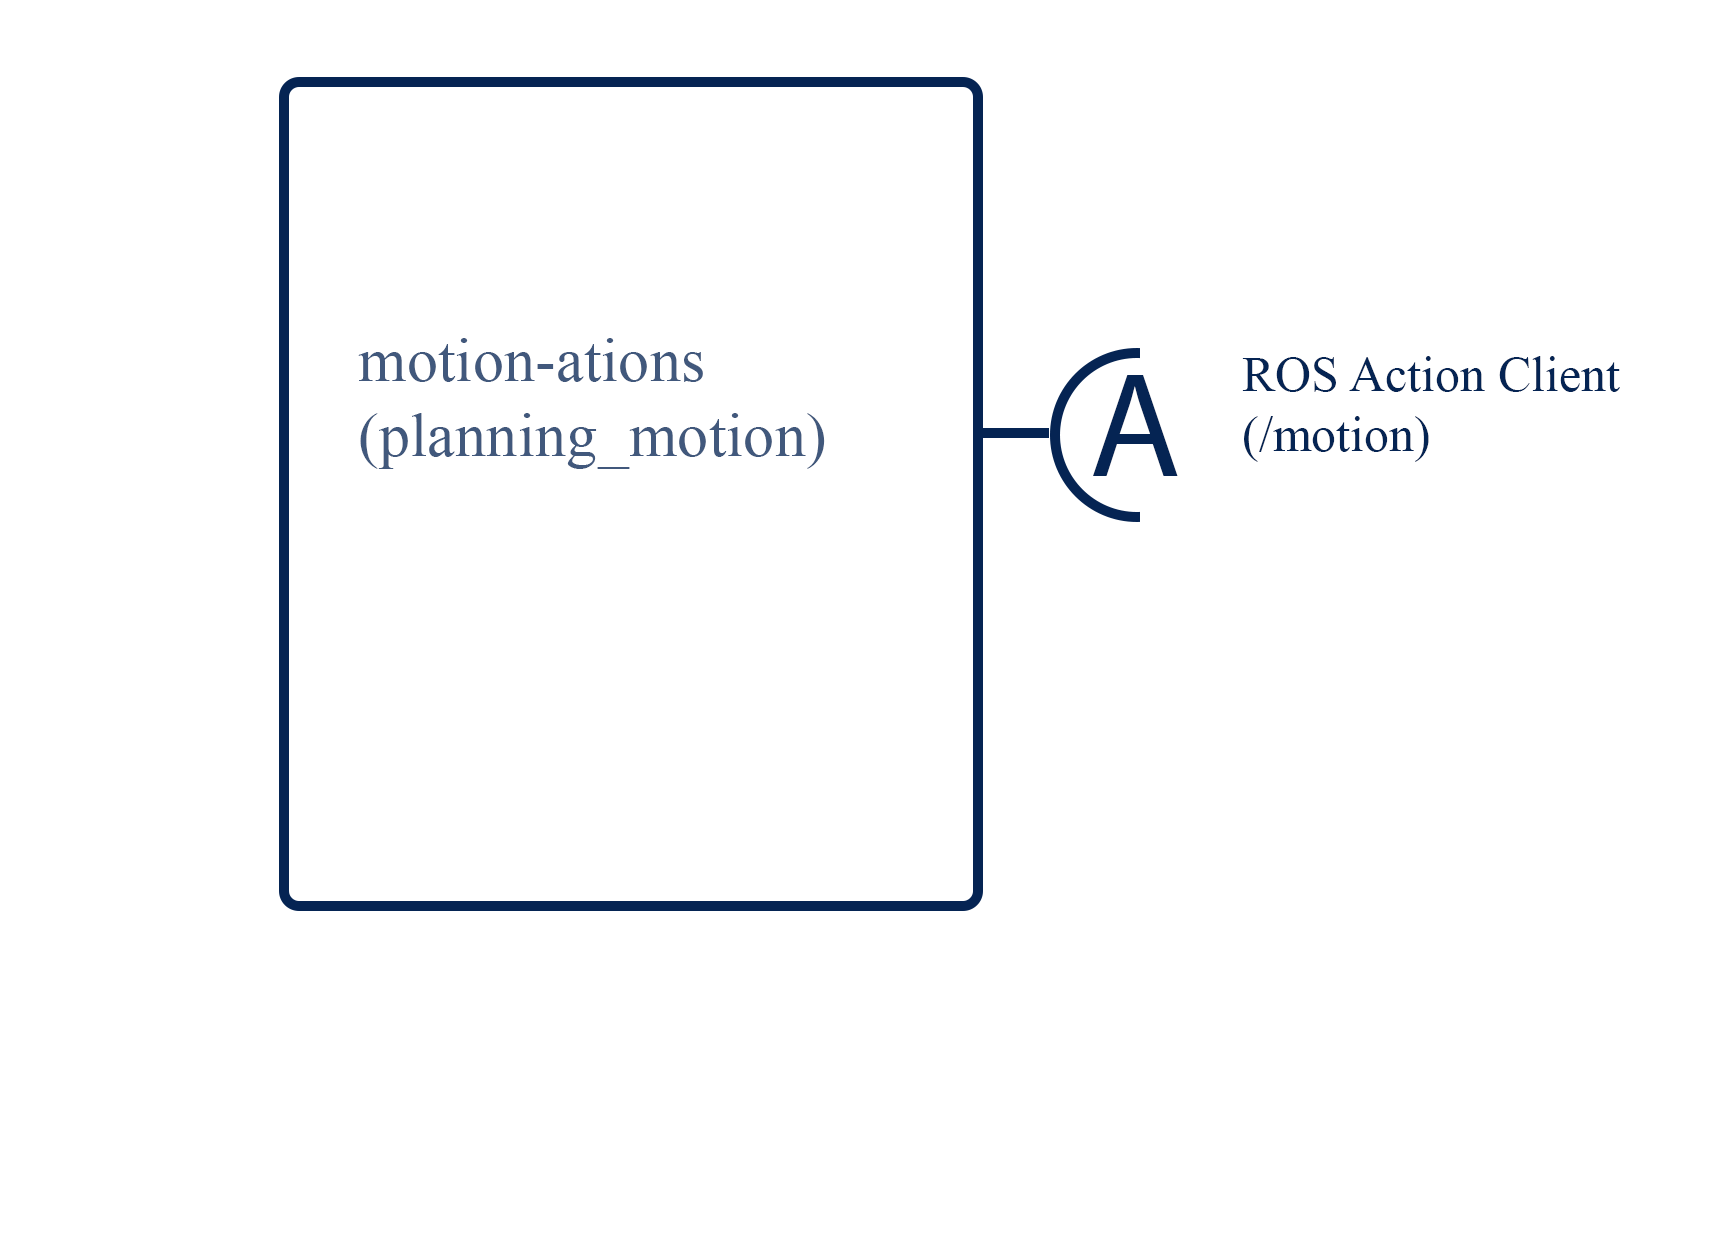
\includegraphics[width=0.6\textwidth]
        {img/motion.png}
        \caption{} Architektur der Quellcode-Datei motion-actions.lisp}
\end{figure}


\subsection{API}
\chapterauthor{Kevin Störmer}
\subsubsection{Actionclients}
1. '/motion' \\
Bewegt die Arme des Pr2 entweder in die Home-Position oder zu einem bestimmten Punkt.
\subsection{Beschreibung des Teilsystems}
\subsubsection{\"Ubersicht}
\chapterauthor{Kevin Störmer}
Die Die Quellcode-Datei 'motion-actions' im Paket 'planning\_motion'  ist ausschliesslich für die Kommunikation mit Gruppe Motion zuständig. Dabei wird die Action '/motion' einmal für die Home-Position des Pr2 und zum Bewegen des Armes zu einem bestimmten Punkt und zum greifen genutzt.


\subsubsection{call-Motion-\\
Move-Arm-Homeposition()}
\chapterauthor{Vanessa Hassouna und Hauke Tietjen}
\begin{verbatim}
call-Motion-Move-Arm-Homeposition()

Beschreibung: Ruft den Actionserver von Motion auf und gibt 
ihnen den Befehl die Arme in die Homeposition zu fahren.

@return: Succesfull oder Aborted
\end{verbatim}



\subsubsection{call-Motion-\\
Move-Arm-To-Point (point-center-\\of-object \&optional (x 3))
}
\chapterauthor{Vanessa Hassouna und Hauke Tietjen}
\begin{verbatim}
call-Motion-Move-Arm-To-Point (point-center-of-object \&optional (x 3))

Beschreibung: Ruft den Actionserver von Motion auf und gibt
ihnen den Befehl den Arm zu dem point-center-of-object zu fahren. 
Optional kann man den Arm hier auswählen, der bei default der rechte ist.

@param point-center-of-object &optional (x 3)
@return: Succesfull oder Aborted
\end{verbatim}

\newpage
\section{Die Quellcode-Datei: movement.lisp (planning\_move)}
\subsection{Architekturbild}
\chapterauthor{Kevin Störmer}


\begin{figure}[!htb]
        \center{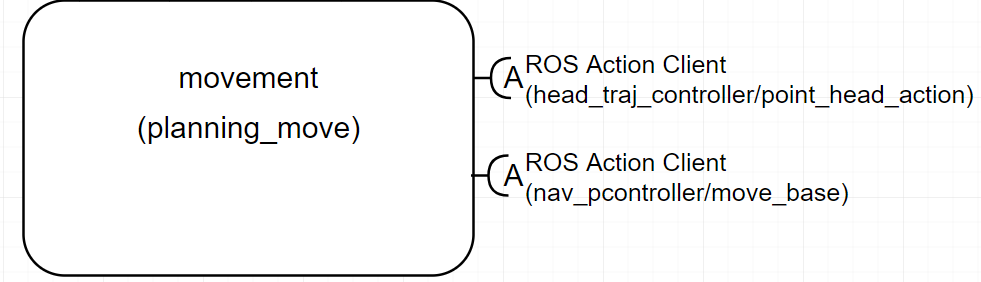
\includegraphics[width=0.8\textwidth]
        {img/diag_planning_move.png}
        \caption{} Architektur der Quellcode-Datei movement.lisp}
\end{figure}


\subsection{API}
\chapterauthor{Kevin Störmer}
\subsubsection{Actionclients}
1. 'head\_traj\_controller/point\_head\_action' \\
Bewegt den Kopf des Pr2 in Richtung eines Punktes.\\ \\
2. 'nav\_pcontroller/move\_base' \\
Bewegt die Basis des Pr2 in Richtung eines Punktes.
\subsection{Beschreibung des Teilsystems}

\subsubsection{\"Ubersicht}
\chapterauthor{Kevin Störmer}
Die Quellcode-Datei actions.lisp im Paket 'planning\_motion'  ist ausschliesslich für die Kommunikation mit Gruppe Motion zuständig. Dabei wird die Action '/motion' einmal für die Home-Position des Pr2 und zum Bewegen des Armes zu einem bestimmten Punkt genutzt.



\subsubsection{move-head (x y z)}
\chapterauthor{Kevin Störmer}

\noindent
\begin{minipage}{\linewidth}
\begin{lstlisting}
(defun move-head (x y z)
   "Moving robot head via head_traj_controller/point_head_action. X Y Z are treated as coordinates."
     (let ((actionclient 
            (actionlib:make-action-client "head_traj_controller/point_head_action" "pr2_controllers_msgs/PointHeadAction")))
       (loop until
            (actionlib:wait-for-server actionclient))
       (let ((point-to-look-at 
            (cl-transforms-stamped:to-msg 
            (cl-transforms-stamped:make-point-stamped "base_link" 0 
                                                       (cl-transforms:make-3d-vector x y z)))))
           (let ((actiongoal 
               (actionlib:make-action-goal actionclient target point-to-look-at)))
               (actionlib:call-goal actionclient actiongoal)))))
\end{lstlisting}
\end{minipage}

Die Funktion 'move-head' bekommt als \"Ubergabeparameter Koordinaten (x y z) welche vorgeben sollen, in welche Richtung der Kopf des Pr2 bewegt wird.\\
Zuerst wird ein neuer Actionclient, für die 'head\_traj\_controller/point\_head\_action' Action erstellt. Anschliessend soll in einem Loop solange gewartet werden, bis der Actionsserver gestartet wurde. Ist dies der Fall, wird eine neue Message erstellt, welche einen Punkt auf Basis der \"ubergebenen Koordinaten, in Relation zum Frame 'base\_link', enth\"alt. Diese wird dann in ein neues Actiongoal gefasst und an den Actionserver geschickt, welcher den Kopf des Pr2 dann in Richtung der Koordinaten bewegen wird.




\subsubsection{move-Base-To-\\
Point-Safe (x y z angle))
}
\chapterauthor{Vanessa Hassouna}
\begin{verbatim}
move-Base-To-Point-Safe (x y z angle)

Beschreibung: Hier wird move-Base-To-Point aufgerufen, jedoch 
bevor dies mit den gegeben Punkten passiert, fährt er in
eine von Uns definierte Position. Das stellt sicher, dass er nicht gegen Kanten stößt.
 
@param: x y z angle
@return: Succesfull oder Aborted
\end{verbatim}


\subsubsection{move-Base-To-\\
Point (x y z angle)}
\chapterauthor{Vanessa Hassouna}
\begin{verbatim}
move-Base-To-Point (x y z angle)

Beschreibung: Anhand des  "nav\_pcontroller/move\_base" 
wird die Basis bewegt. Der Punkt und die Rotation sind in Frame "map" anzugeben.

@param: x y z angle
@return: Succesfull oder Aborted
\end{verbatim}



\subsubsection{move-Robo-Into\\
-Homeposition ()}
\chapterauthor{Vanessa Hassouna}
\begin{verbatim}
move-Robo-Into-Homeposition ()

Beschreibung: move-Base-To-Point wird aufgerufen mit 
von uns vordefinierten Punkten die als Homeposition  definiert sind.

@return: Succesfull oder Aborted
\end{verbatim}


\subsubsection{init-Robo-Moving ()}
\chapterauthor{Vanessa Hassouna}
\begin{verbatim}
init-Robo-Moving ()

Beschreibung: Eine Hilfsfunktion die dazu dient, die Initialisierung in der Simulation
zu Übernehmen.

@return: Succesfull oder Aborted
\end{verbatim}

\subsubsection{init-Action-Client-Base ()}
\chapterauthor{Vanessa Hassouna}
\begin{verbatim}
init-Action-Client-Base ()

Beschreibung: Eine Hilfsfunktion die dazu dient, den Action-Client zu initialisieren.

@return: Succesfull oder Aborted
\end{verbatim}


\subsubsection{get-Action-Client-Base ()}
\chapterauthor{Vanessa Hassouna}
\begin{verbatim}
get-Action-Client-Base ()

Beschreibung: Eine Hilfsfunktion die dazu dient, den Action-Client zu erhalten.

@return: Succesfull oder Aborted
\end{verbatim}






\newpage
\section{Die Quellcode-Datei: external-logic.lisp (planning\_logic)}
\subsection{Architekturbild}
\chapterauthor{Vanessa Hassouna}


\begin{figure}[!htb]
        \center{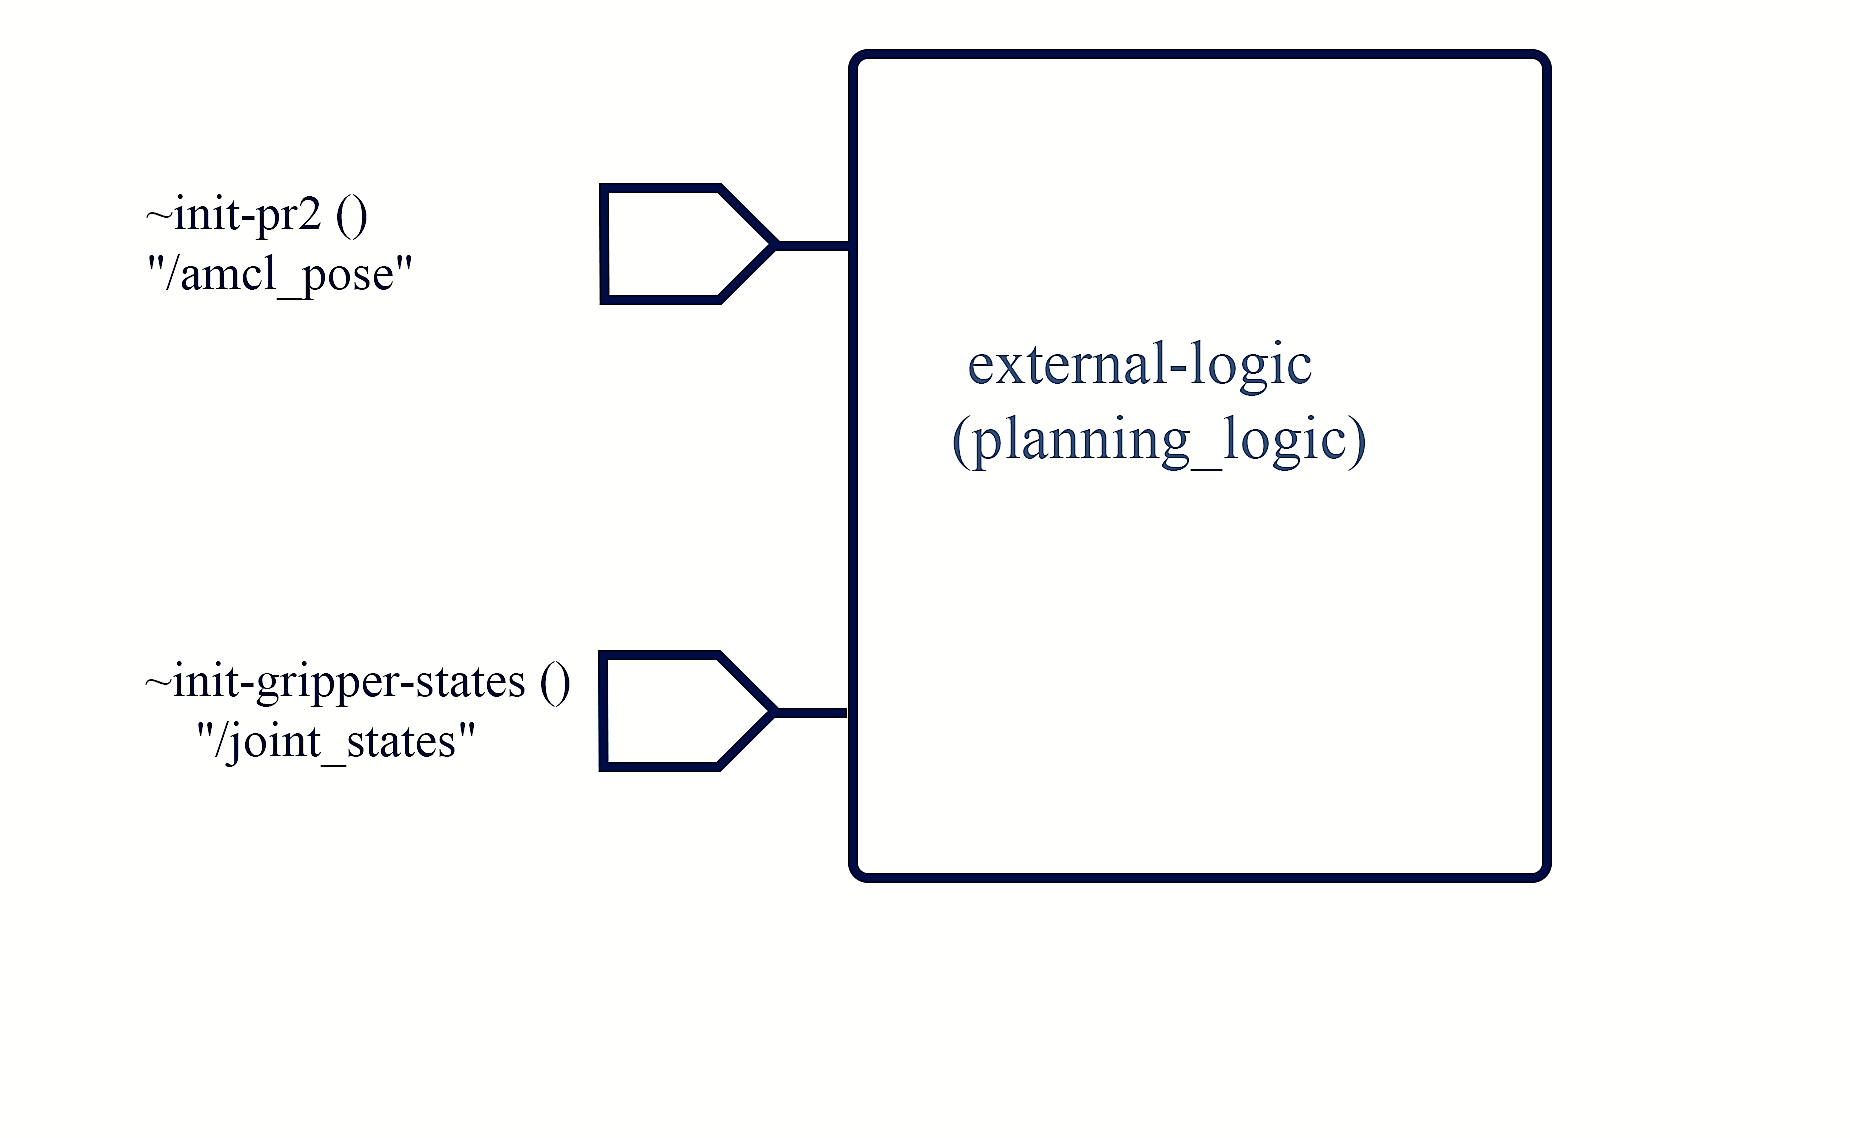
\includegraphics[width=0.8\textwidth]
        {img/externallogic.png}
        \caption{} Architektur der Quellcode-Datei movement.lisp}
\end{figure}


\subsection{API}
\chapterauthor{Vanessa Hassouna}
\subsubsection{Topics}
1. 'joint\_states' \\
Hört auf den Topic und speichert die Werte des Grippers.\\
 %vielleicht willst du hier was schreiben?
 
2. 'robot\_pose' \\
Gibt uns die Position des Roboters.
\subsection{Beschreibung des Teilsystems}

\subsubsection{\"Ubersicht}
\chapterauthor{Vanessa Hassouna}
Die Quellcode-Datei external-logic.lisp im Paket 'planning\_logic'  ist für Funktionen gedacht die außerhalb der anderen Pakete funktionieren und eine Logik beinhalten die nicht zusätzlichen Platz in der main.lisp einehm soll.



\subsubsection{transformation-Vision-Point (pose amount\\
\&optional (endFrame "/base\_footprint")}
\chapterauthor{Vanessa Hassouna}
\begin{verbatim}
transformation-Vision-Point (pose amount &optional (endFrame "/base\_footprint")

Beschreibung: Das gegeben Objekt wird von dem ausgehenden Frame 
in ein optionalen Frame umgewandelt(bei default ist dieser base\footprint)

@param: pose, amount und optional endFrame
@return: Liefert eine transformierte tf-point-stamped
\end{verbatim}




\subsubsection{catch-Transformation \\
(transform-listener tf-point-stamped endFrame)}
\chapterauthor{Vanessa Hassouna}
\begin{verbatim}
catch-Transformation (transform-listener tf-point-stamped endFrame)

Beschreibung: Hier findet die eigentliche transformation statt.

@param: transform-listener tf-point-stamped endFrame
@return: Liefert eine transformierte tf-point-stamped
\end{verbatim}


% KOMMT NOCH(defun let-Robo-Try-To-Poke (point-for-motion number-for-arm)
%KOMMT NOCH (defun try-To-Poke-Different-Location(point-for-motion number-for-arm)


\subsubsection{should-Robo-Use-Left-Or-Right-Arm(pose amount \\
\&optional (endFrame "/base\_footprint"))}
\chapterauthor{Vanessa Hassouna}
\begin{verbatim}
should-Robo-Use-Left-Or-Right-Arm (pose amount &optional (endFrame "/base\_footprint"))

Beschreibung: Anhand der Y-Achse entscheidet der Roboter
ob er den linken oder rechten Arm bewegen soll.

@param: pose object-number &optional endFrame
@return: 3 oder 2 (3 = links 2 = Rechts)
\end{verbatim}


\subsubsection{disassemble-Vision-Call (visionclouds)}
\chapterauthor{Vanessa Hassouna}
\begin{verbatim}
disassemble-Vision-Call (visionclouds)

Beschreibung: Extrahiert alle Informationen aus der Visioncloud und speichert
 normal\_features, color\_features, object\_amount und object\_pose auf den Param-Server.
 
@param: visionclouds
@return: object\_pose
\end{verbatim}



\subsubsection{set-Params-Features \\
(normal-s color-s normal-e color-e amount)}
\chapterauthor{Vanessa Hassouna}
\begin{verbatim}
set-Params-Features (normal-s color-s normal-e color-e amount)

Beschreibung: Hilfsfunktion für disassemble-Vision-Call um aus
normal\_features und color\_features Konkateniert ein features-X zu erstellen. 

@param: normal-s color-s normal-e color-e amount
@return: Nil
\end{verbatim}


\subsubsection{init-pr2()}
\chapterauthor{Vanessa Hassouna}
\begin{verbatim}
init-pr2 ()

Beschreibung: Hört auf ein Topic Namens "/robot_pose" und bindet die Information.

@return: geometry_msgs/Pose
\end{verbatim}

\subsubsection{pose-cb (msg)}
\chapterauthor{Vanessa Hassouna}
\begin{verbatim}
pose-cb (msg)

Beschreibung: Rückrufende Funktion. Der Wert von msg wird als 
fluent *pr2-pose* gespeichjert.

@param: msg
@return: geometry_msgs/Pose
\end{verbatim}

\subsubsection{move-pr2 (x y z)}
\chapterauthor{Vanessa Hassouna}
\begin{verbatim}
move-pr2 (x y z)

Beschreibung: Ruft move-Base-To-Point-Safe mit angle-From-Pr2-Pose-To-Point auf.

@param: x y z 
@return: Succesfull oder Aborted
\end{verbatim}

\subsubsection{angle-From-Pr2-Pose-To-Point (x-goal y-goal z-goal)}
\chapterauthor{Vanessa Hassouna}
\begin{verbatim}
angle-From-Pr2-Pose-To-Point (x-goal y-goal z-goal)

Beschreibung: Berechnet von der aktuellen Position des Roboters um wie viel Grad er 
sich drehen muss um zu einem Punkt zu fahren, dafür wurde unter anderem das Packet
"Cram-Language" mit der Funktion atan benutzt. Da das Bewegen des Pr2 in dem 
Frame "map" stattfindet, wurde hier zusätzlich noch die aktuelle Drehung des 
Pr2 in der Welt festgestellt und diese dann mit dem Grad um wie viel er sich 
drehen muss gegengerechnet, sodass am Ende ein Angle produziert wird, der 
innerhalb des Frames "map" funktioniert. 

@param: x-goal y-goal z-goal 
@return: angle 
\end{verbatim}


\subsubsection{try-To-Poke-Different-Location\\
(point-for-motion number-for-arm)}
\chapterauthor{Vanessa Hassouna}
\begin{verbatim}
 try-To-Poke-Different-Location(point-for-motion number-for-arm)

Beschreibung: Die Funktion lässt den Roboter anhand vorgegebener Zahlen seinen Winkel sowie seine Position ändern, wenn er das Objekt nicht erreichen kann.

@param: point-for-motion number-for-arm
@return: T oder Nil


\end{verbatim}

























\newpage
\section{Nutzungsbeschreibung}

\subsection{Installation und Ausführung von Planning}

\subsubsection{Installation}
\chapterauthor{Vanessa Hassouna}
\begin{itemize}


\item[a] Laufen alle anderen Systeme (Vision,Knowledge und Motion) muss man für Planning folgendes Repository hinzufügen: \url{https://github.com/menanuni/planning_suturo_1718.git}. 

\item[b] Hat man erfolgreich mit \textit{catkin build} seine Arbeitsumgebung vollständig bauen können, muss man CRAM installieren \url{http://cram-system.org/installation}.

\item[c] Nun wird die Entwicklungsumgebung installiert mit: \textbf{sudo apt-get install emacs}. Achtung: Bei der Verwendung von Ubuntu 14.04 muss der neueste Lisp 'compiler' noch hinzugefügt werden \url{https://sourceforge.net/projects/sbcl/files/sbcl/1.3.1/
} (meistens x86-64 Version). Diese Datei entpacken und im Terminal (im richtigen Ordner) den Befehl: \textbf{sh install.sh} eingeben.
\end{itemize}

\subsubsection{Ausführung}
\chapterauthor{Vanessa Hassouna}
\begin{itemize}

\item Zuerst muss im Terminal \textbf{roslisp\_repl} eingeeben werden, daraufhin startet emacs. 

\item Nun wird in der Repl (dort wo cl-user steht) ein \textbf{,} (also das Komma auf der Tastertur) eingegeben.

\item Darauf folgt \textbf{r-l-s} mit \textbf{enter} und nun muss \textbf{planning\_main\_programm} mit \textbf{enter} bestätigt werden.

\item Zum Schluss wird noch in dem cl-user Fenster \textbf{(planning-main-programm::main)} eingegeben und mit \textbf{enter} bestätigt (die Klammern gehören auch dazu).
\end{itemize}


\subsection{Installation und Ausführung von Motion}

\subsubsection{Installation}
\chapterauthor{RH, MB}
\begin{itemize}


\item[a] Zunächst müssen folgende Repositories in den source-Ordner des Workspaces hinzugefügt werden:  \\
\url{https://github.com/menanuni/motion_suturo_1718} \\
\url{https://github.com/menanuni/msgs_suturo_1718} \\
\url{https://github.com/menanuni/knowledge_suturo_1718} \\

\item[b] Es muss das MoveIt Framework installiert werden, dazu im Terminal: \\
\textit{sudo apt-get update} \\
\textit{sudo apt-get install ros-indigo-moveit} \\
\textit{echo  \grqq{}source /opt/ros/indigo/setup.bash\grqq{} \textgreater\textgreater \textasciitilde{ }/.bashrc} \\

\item[c] Jetzt kann das System über \textit{catkin build} gebaut werden.

\end{itemize}

\subsubsection{Ausführung}
\chapterauthor{Roman Haak}
\begin{itemize}

\item Zunächst muss über den Befehl \textit{roslaunch kitchen\_model\_export knowledge\_export\_service.launch} ein Teilsystem von \textit{Knowledge} gestartet werden.

\item Anschließend kann unser Knoten über \textit{roslaunch motion motion\_main\_start.launch} gestartet werden, falls er im Kontext einer Simulation ausgeführt werden soll, bzw. \textit{roslaunch motion motion\_main\_start\_real\_pr2.launch}, falls der Knoten auf dem PR2 ausgeführt werden soll.

\item Dann können Befehle an den Actionserver unseres Knotens über das Topic \textit{/moving/goal} abgesetzt werden. Zur Erläuterung des Actionservers siehe Dokumentation der Gruppe \textit{motion}.
\end{itemize}


\subsection{Installation und Ausführung von Vision}

\subsubsection{Installation}
\chapterauthor{Alexander Link}

\textbf{Voraussetzungen}

\begin{itemize}
\item Ubuntu 14.04
\item ROS Indigo
\item Catkin tools
\item Gazebo 2.2.x
\end{itemize}

\textbf{.bashrc}

Folgendes muss zur .bashrc (oder zshrc) hinzugefügt werden:
\begin{itemize}
\item \textit{export KINECT1=true}
\item \textit{export GAZEBO\_MODEL\_PATH= \$HOME/catkin\_ws/vision\_suturo\_1718/vision/models}
\item \textit{export GAZEBO\_RESOURCE\_PATH= \$HOME/catkin\_ws/vision\_suturo\_1718/vision/worlds}
\end{itemize}

\textbf{Setup}

\begin{itemize}
\item gazebo installieren: \textit{sudo apt-get install ros-indigo-pr2-simulator}

\item Sollten Probleme auftreten, könnte dies durch ein Update von gazebo auf v2.2.6 gelöst werden:
\\
\textit{sudo sh -c 'echo "deb http://packages.osrfoundation.org/gazebo/ubuntu trusty main" > /etc/apt/sources.list.d/gazebo-latest.list'}
\\
\textit{wget http://packages.osrfoundation.org/gazebo.key -O - | sudo apt-key add -}
\\
\textit{sudo apt-get update}

\item Folgende Pakete in den src-Ordner eines catkin workspaces klonen:\\
        \textbf{vision\_suturo\_1718} (this package) \\
        \textbf{msgs\_suturo\_1718}
\item Erst "\textit{catkin build object\_detection}" nutzen, um die messages zu bauen.
\item Dann "\textit{catkin build}" benutzen, um alles andere zu bauen.

\end{itemize}

\textbf{Kinect benutzen}
\begin{itemize}
\item \textit{sudo apt install ros-indigo-freenect-launch freenect libfreenect-bin}
\item \textit{roslaunch freenect\_launch freenect-registered-xyzrgb.launch}
\item (Optional) \textit{roslaunch vision vision\_kinect.launch}
\end{itemize}

\textbf{Dateien speichern}

    \textit{rosrun pcl\_ros pointcloud\_to\_pcd input:=/camera/depth\_registered/point}


\subsubsection{Ausf\"uhrung}
\chapterauthor{Alexander Link}

\textbf{vision\_main/objectPoint}
\begin{itemize}
\item Liefer einen PointStamped und einen Fehlercode zurück
\item Nimmt keine Argumente
\item Benutzt VisObjectInfo.srv
\end{itemize}
\textbf{vision\_main/objectPose (WIP)}
\begin{itemize}
\item Gibt einen bool zur\"uck, der angibt, ob ein Objekt steht oder liegt, zusammen mit einem String f\"ur weitere Informationen.
\item Nimmt keine Argumente
\item Benutzt GetObjectInfo.srv 
\end{itemize}

\textbf{rosservice}

Unsere Services k\"onnen auch manuell abgerufen werden: \\

\textit{rosservice call vision\_main/objectPoint} \\

oder \\

\textit{rosservice call vision\_main/objectPose}

\subsection{Installation und Ausführung von Knowledge}

\subsubsection{Installation}
\chapterauthor{Alexander Haar}

\begin{itemize}
\item[1.] Java8 installieren:$ https://wiki.ubuntuusers.de/Java/Installation/Oracle_Java/Java_8/ $Wichtig JDK
\item[2.] Repo clonen und bauen
\item[3.] Die folgenden Schritte ausführen: $http://knowrob.org/installation/workspace$
\end{itemize}

\subsubsection{Ausführung}
\chapterauthor{Alexander Haar}

Um alle wichtigen Knoten zu starten muss einfach der Befehl \textit{roslaunch knowledge knowledge\_main.launch} ausgeführt werden. Es wird eine json\_prolog- Node, der PokePositon-Service und der GetFixedKitchenModel- Service gestartet.
\end{document}

